\documentclass[journal,12pt,onecolumn]{IEEEtran}
\usepackage[utf8]{inputenc}   % Codificación de entrada
\usepackage[T1]{fontenc}      % Codificación de fuente
\usepackage[spanish,es-tabla]{babel}   % Idioma español
\usepackage{lmodern}          % Fuente moderna
\usepackage{amsmath, amssymb} % Matemáticas y símbolos
\usepackage{graphicx} 		  % Gráficos e imágenes
\graphicspath{{img/}{tablas/}{portada/}}  % Las imágenes se buscarán en la carpeta "img"
\usepackage{longtable}      % Para tablas que se extienden en varias páginas
\usepackage{tabularx}	% Tablas avanzadas
\usepackage{threeparttable}
\usepackage{hyperref}	% Hipervínculos
\usepackage{float}
%-------------------------------------------
% Otros paquetes útiles (personaliza según tus necesidades)
%-------------------------------------------
\usepackage{caption}
\usepackage{subcaption}
\usepackage{xcolor}
\usepackage{setspace}

%-------------------------------------------
% Comandos personalizados
\renewcommand{\listtablename}{Índice de tablas}
\renewcommand{\appendixname}{Anexos}
\definecolor{colorreferences}{RGB}{48,134,3}

% Metadatos del PDF
\hypersetup{
	unicode=true,
	hidelinks,
	colorlinks=true,       % false: boxed links; true: colored links
	linkcolor=black,          % color of internal links (change box color with linkbordercolor)
	citecolor=colorreferences,        % color of links to bibliography
	filecolor=magenta,      % color of file links
	urlcolor=blue,           % color of external links
	linkbordercolor={0 0 0}
}
%-------------------------------------------
% Inicio del documento
%-------------------------------------------
\begin{document}

% Aquí se encuentra el archivo con la portada
\begin{titlepage}
	\centering
	%-------------------------------------------
	% Logos en una tabla: izquierda, centro y derecha
	\begin{tabular}{@{}p{0.3\textwidth} p{0.3\textwidth} p{0.3\textwidth}@{}}
		
\includegraphics[height=2cm]{tecnm} & 
		\centering 
\includegraphics[height=1.5cm]{SEP} & 
		\raggedleft 
\includegraphics[height=2cm]{ith.jpg} \\
	\end{tabular}
	
	\vspace{2em}
	
	\noindent
	%-------------------------------------------
	%	Información institucional y académica (esquina superior izquierda)
	\begin{minipage}[t]{0.48\textwidth}
		\raggedright
		\small \textbf{%
			Instituto Tecnológico de Hermosillo\\
			Materia: Robótica\\
			Profesor: Medina Gil Lamadrid, Jesús Iván%
		}
	\end{minipage}%
	\hfill
	%	fecha actual (esquina superior derecha), en letras pequeñas y en negrita.
	\begin{minipage}[t]{0.48\textwidth}
		\raggedleft
		\small \textbf{\today}
	\end{minipage}
	
	\vspace{2em}
	
	%-----------------------------------------
	% Unidad y Título de la tarea en letras grandes y en negrita
	{\large \textbf{Unidad 1: Morfología del robot}}\\
	{\Huge \textbf{Tipos de Sensores}}
		
	\vspace{1em}
	
	%---------------------------------------
	% Tabla con la información del equipo
	%---------------------------------------
	% Encabezado del equipo
	\begin{center}
		{\Large \textbf{Equipo 6}}
	\end{center}
	
	\vspace{1em}
	
	% Tabla de integrantes:
	% Cada fila contiene: foto (columna izquierda) y datos del integrante (columna derecha)
	\begin{center}
		\begin{tabular}{c c}
			\begin{tabular}{c}
				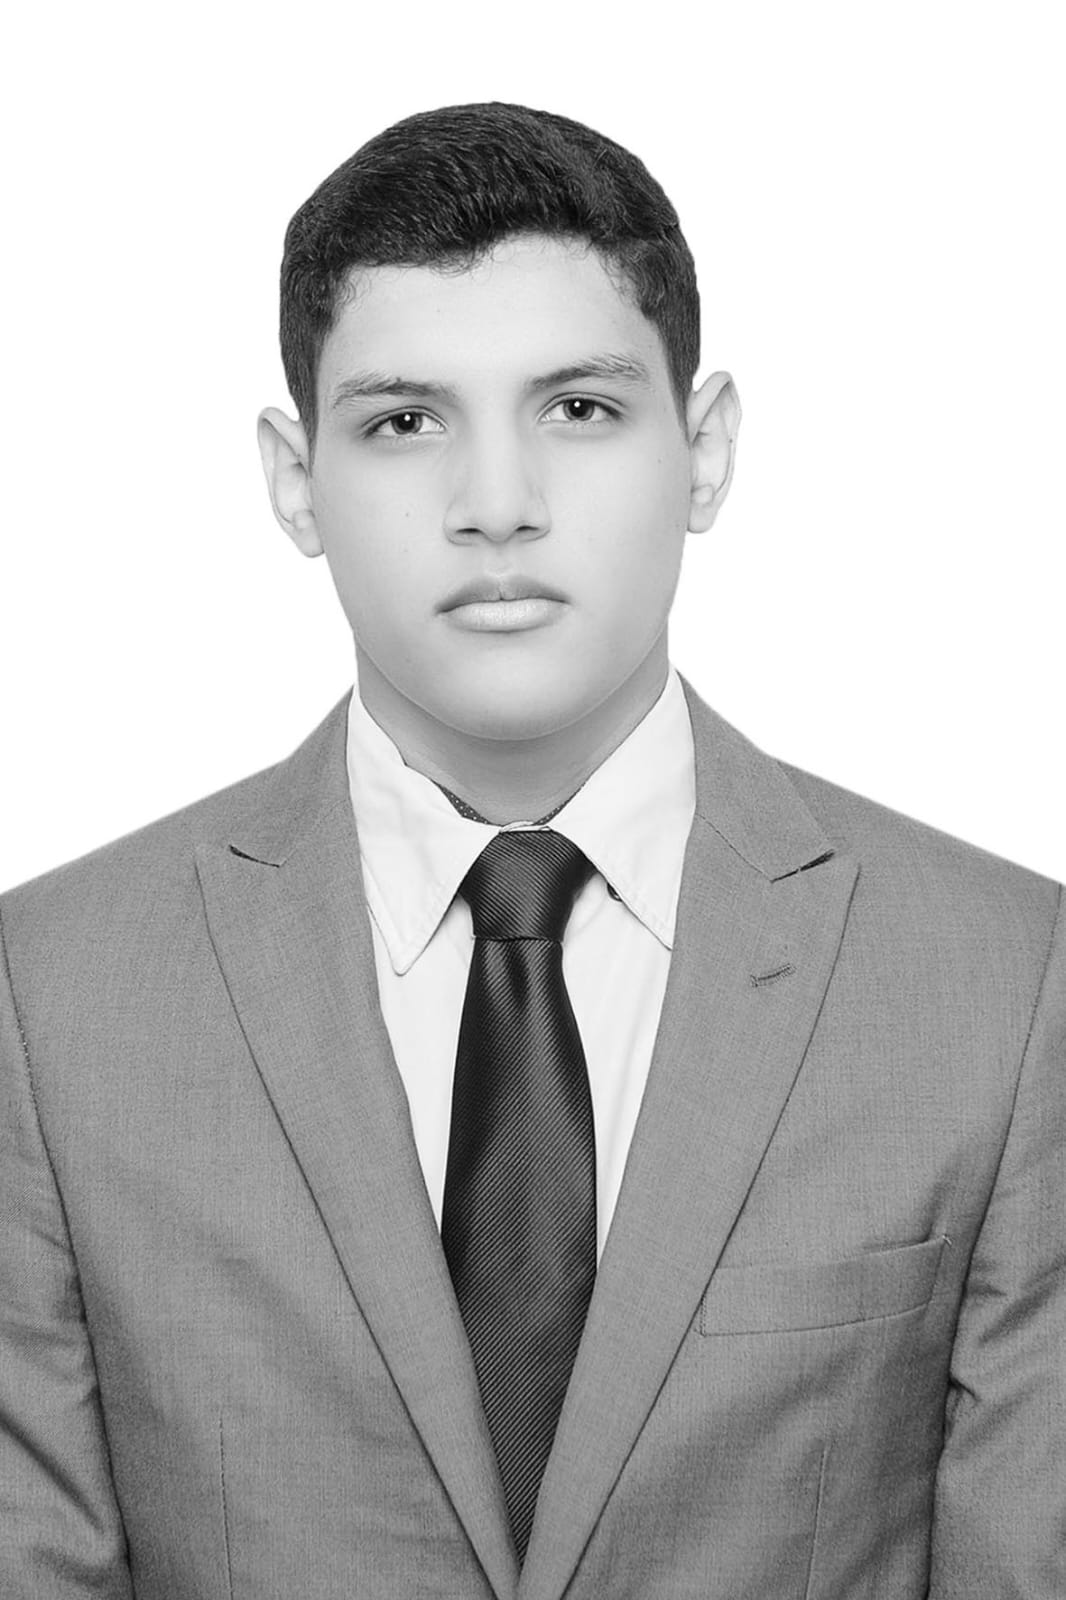
\includegraphics[height=3cm]{alexander.jpg} \\
				\textbf{Hernandez Dominguez },\\ Olinsser Alexander \\ \texttt{l21330599@hermosillo.tecnm.mx} \\ 
			\end{tabular} &
			\begin{tabular}{c}
				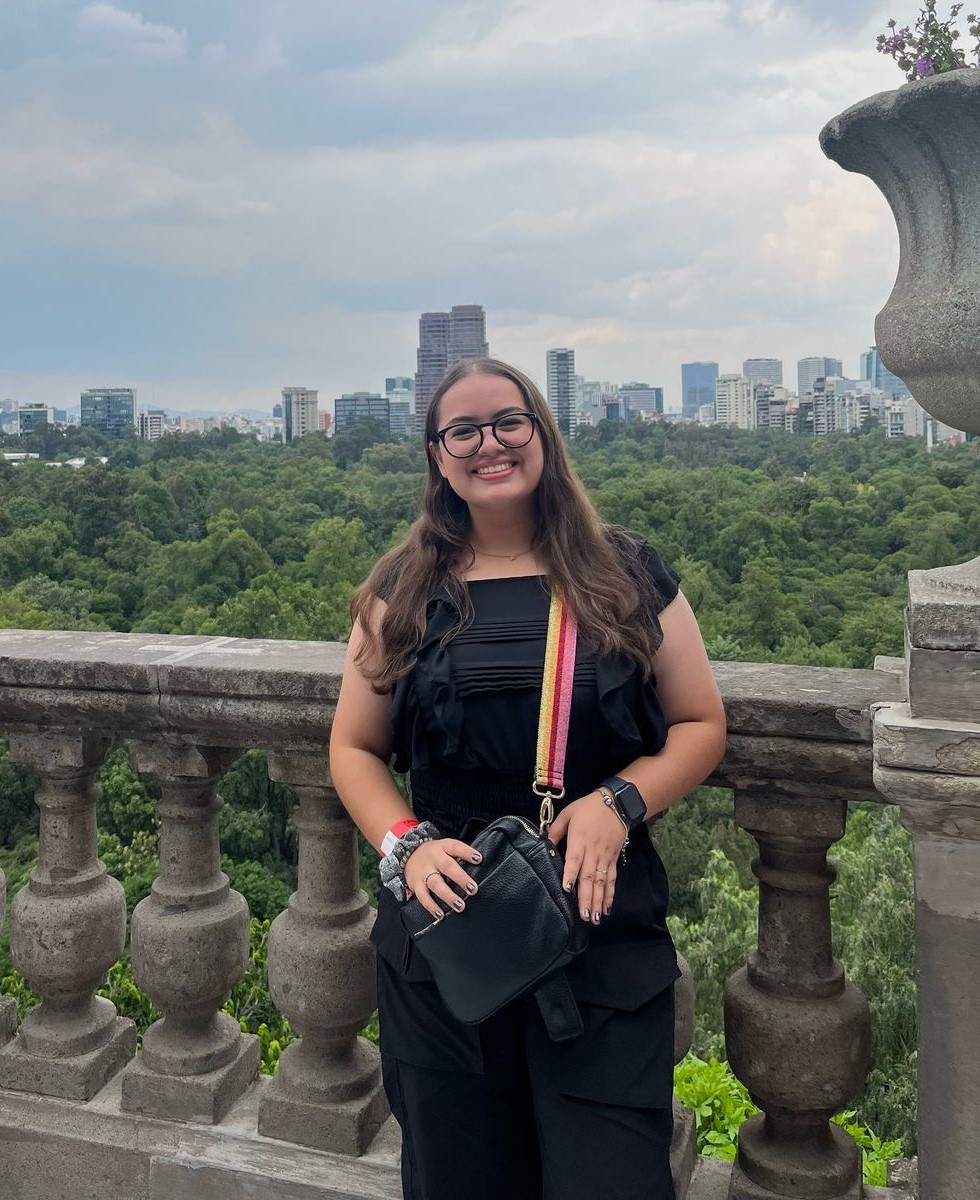
\includegraphics[height=3cm]{iliana.jpg} \\
				\textbf{Medina de la Rocha,}\\ Iliana \\ \texttt{l21330629@hermosillo.tecnm.mx} \\
			\end{tabular} \\ \vspace{2em}
			\begin{tabular}{c}
				
\includegraphics[height=3cm]{itzel.jpg} \\
				\textbf{Mesta Valdez,}\\ Itzel \\ \texttt{l21330635@hermosillo.tecnm.mx} \\ 
			\end{tabular} &
			\begin{tabular}{c}
				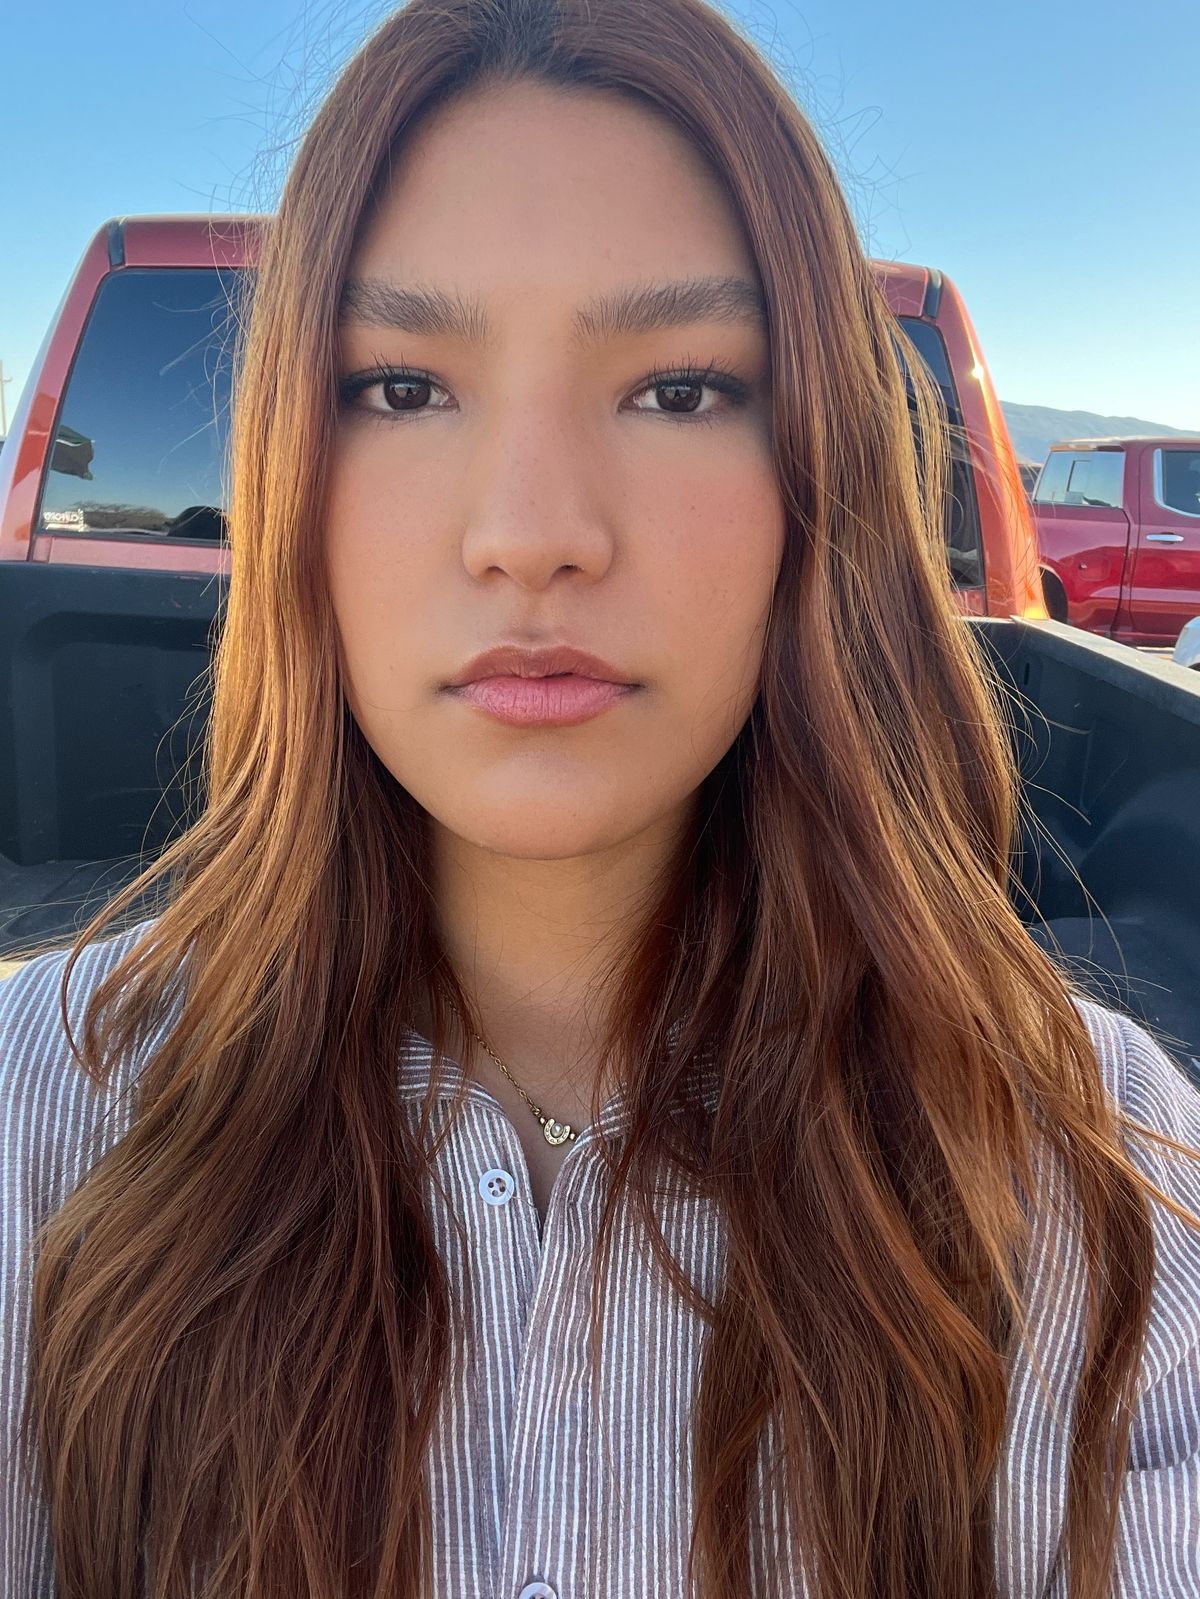
\includegraphics[height=3cm]{luisa.jpg} \\
				\textbf{Santacruz López,}\\ Luisa Fernanda \\ \texttt{l21330691@hermosillo.tecnm.mx} \\ 
			\end{tabular}
		\end{tabular}
	\end{center}

\end{titlepage}

%	Es innecesario poner el índice porque ya aparece en los marcadores del PDF
%\tableofcontents

% Ejemplo de inclusión de una sección (por ejemplo, "introduccion.tex" debe estar en la carpeta "secciones" y se recomienda no usar carácteres especiales (tilde) o espacios)
\section{Ejercicios Denavit Hartenberg}

El presente documento contiene el desarrollo de ejercicios enfocados en la cinemática inversa de dos robots diferentes al robot 1, conforme a las indicaciones establecidas en la tarea. Cada robot fue programado y simulado utilizando MATLAB, generando animaciones que muestran el movimiento del robot al alcanzar un objetivo específico en el espacio.

La cinemática inversa permite determinar los ángulos articulares necesarios para que el efector final del robot alcance una posición deseada. En este reporte se presentan los resultados obtenidos para cada uno de los robots seleccionados, así como las gráficas correspondientes a su trayectoria.

Además, se calcula y analiza el error del objetivo alcanzado, con el fin de evaluar la precisión de cada solución obtenida. Los videos generados durante la simulación han sido guardados y, junto con los archivos de código, pueden encontrarse en el repositorio correspondiente o se adjuntan a este reporte según lo solicitado.
\section{\textbf{Ejercicio1}}
\subsection{\textbf{Robot 2}}

\begin{figure}[h]
	\centering
	\subfloat[Robot 2]{%
		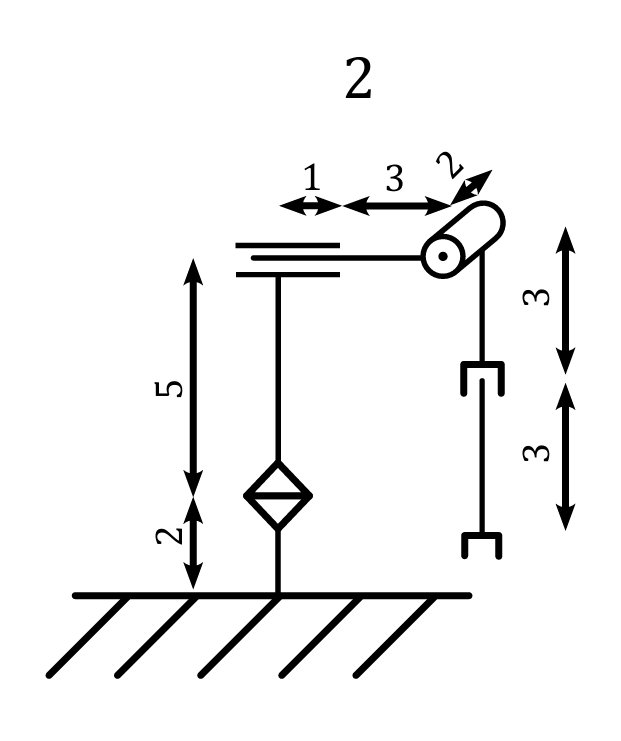
\includegraphics[width=0.4\textwidth]{Ej1.png}%
		\label{fig:Ej1}
	}
	\hfill
	\subfloat[Robot 2 con flechas]{%
		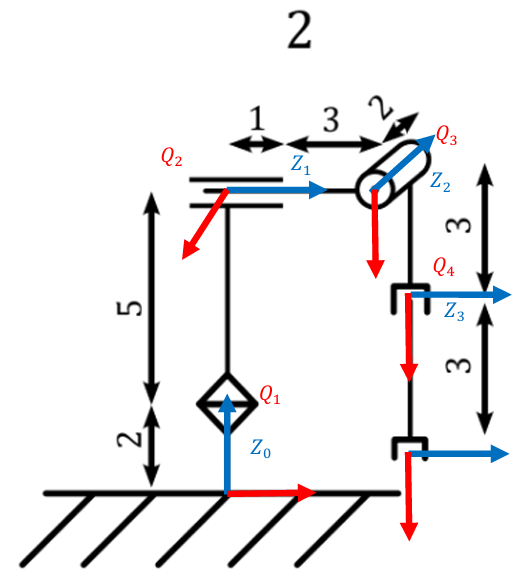
\includegraphics[width=0.4\textwidth]{Ej12.png}%
		\label{fig:Ej1 Flechas}
	}
	\caption{Ejercicio 1: Robot 2}
	\label{fig:Robots}
\end{figure}
\section{\textbf{Ejercicio2}}
\subsection{\textbf{Robot 10}}

\begin{figure}[H]
	\centering
	\subfloat[Robot 10]{%
		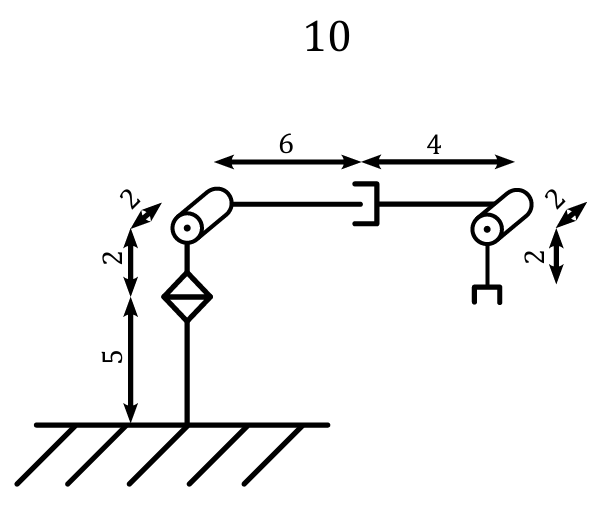
\includegraphics[width=0.4\textwidth]{Ej2.png}%
		\label{fig:Ej2}
	}
	\hfill
	\subfloat[Robot 10 con flechas]{%
		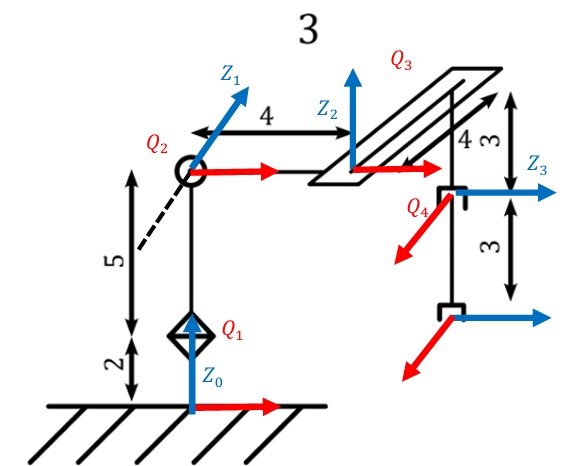
\includegraphics[width=0.45\textwidth]{Ej22.png}%
		\label{fig:Ej22}
	}
	\caption{Ejercicio 2: Robot 10}
	\label{fig:Robot10}
\end{figure}
\begin{figure}[H]
	\centering
	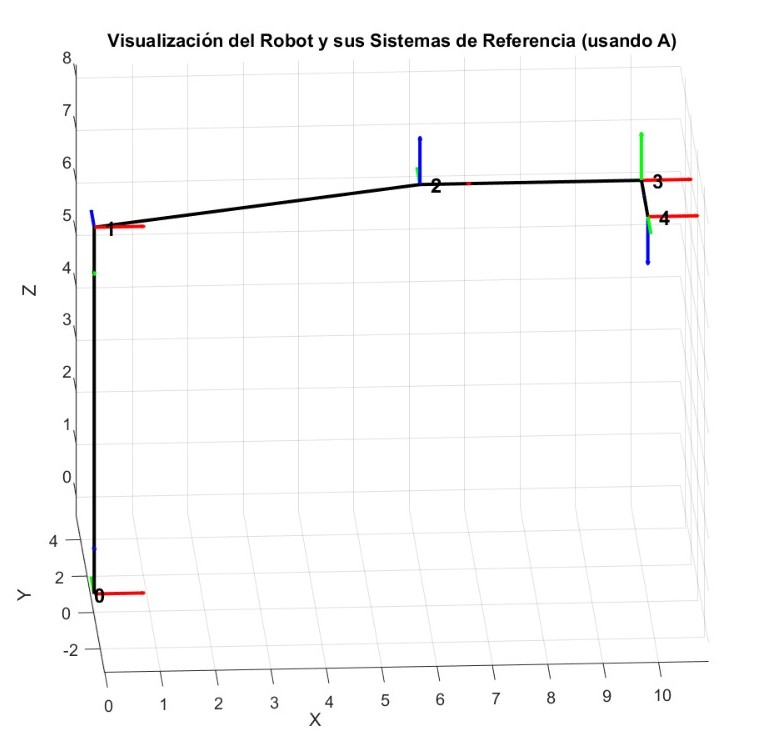
\includegraphics[width=0.7\textwidth]{img/Ej23.jpg}
	\caption{Robot 10 en MATLAB.}
	\label{fig:Robot10matlab}
\end{figure}

\section{\textbf{Ejercicio3}}
\subsection{\textbf{Robot 5}}
\begin{figure}[H]
	\centering
	\subfloat[Robot 5]{%
		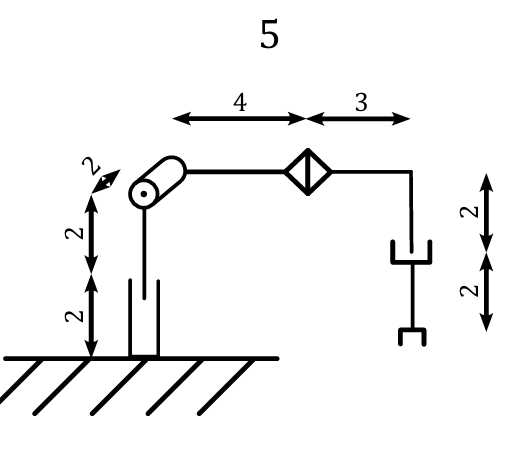
\includegraphics[width=0.4\textwidth]{Ej3.png}%
		\label{fig:Ej3}
	}
	\hfill
	\subfloat[Robot 5 con flechas]{%
		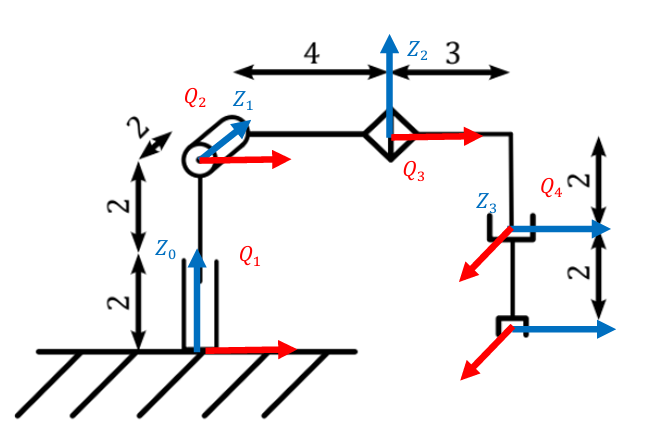
\includegraphics[width=0.4\textwidth]{Ej32.png}%
		\label{fig:Ej32}
	}
	\caption{Ejercicio 3: Robot 5}
	\label{fig:Robot}
\end{figure}
\section{\textbf{Ejercicio4}}
\subsection{\textbf{Robot 7}}

\begin{figure}[H]
	\centering
	\subfloat[Robot 7]{%
		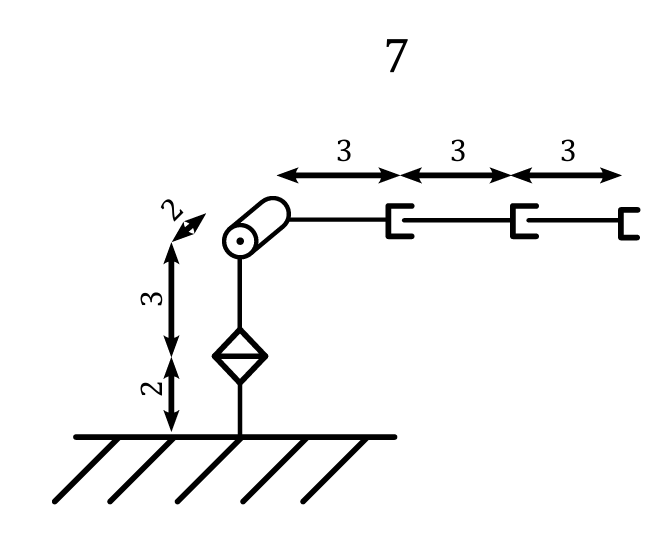
\includegraphics[width=0.4\textwidth]{Ej4.png}%
		\label{fig:Ej4}
	}
	\hfill
	\subfloat[Robot 7 con flechas]{%
		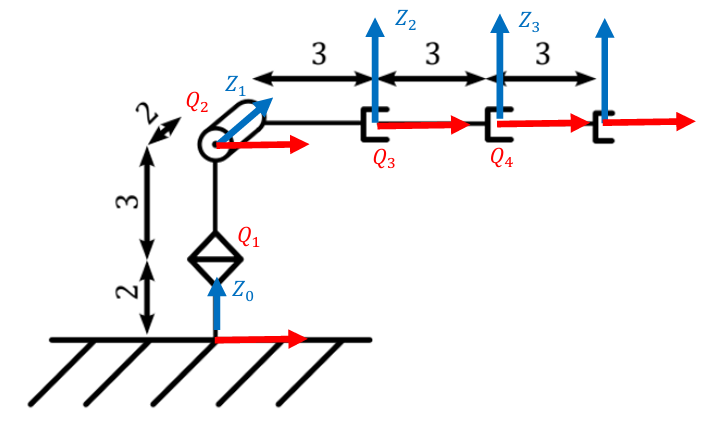
\includegraphics[width=0.45\textwidth]{Ej42.png}%
		\label{fig:ej42}
	}
	\caption{Ejercicio 4: Robot 7}
	\label{fig:Robot7}
\end{figure}


\begin{figure}[H]
\centering
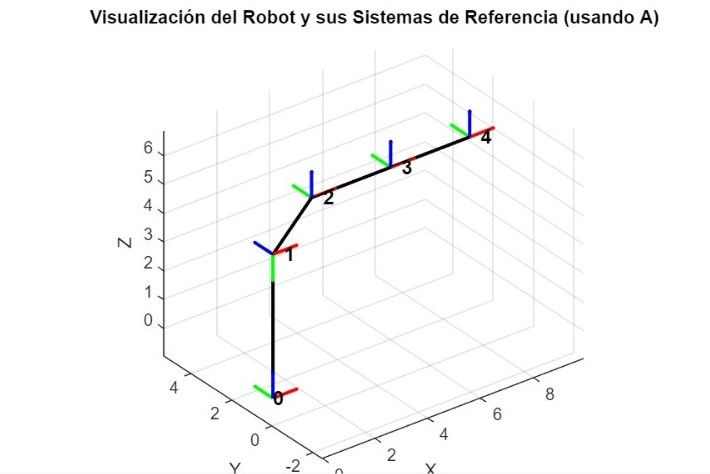
\includegraphics[width=0.7\textwidth]{img/Ej33.jpg}
\caption{Robot 7 en MATLAB.}
\label{fig:Robot7matlab}
\end{figure}
\section{\textbf{Ejercicio5}}
\subsection{\textbf{Robot 9}}

\begin{figure}[H]
	\centering
	\subfloat[Robot 9]{%
		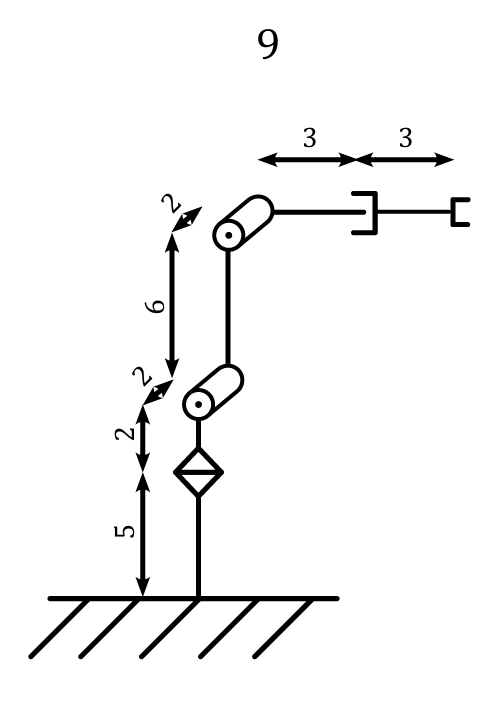
\includegraphics[width=0.4\textwidth]{Ej5.png}%
		\label{fig:Ej5}
	}
	\hfill
	\subfloat[Robot 9 con flechas]{%
		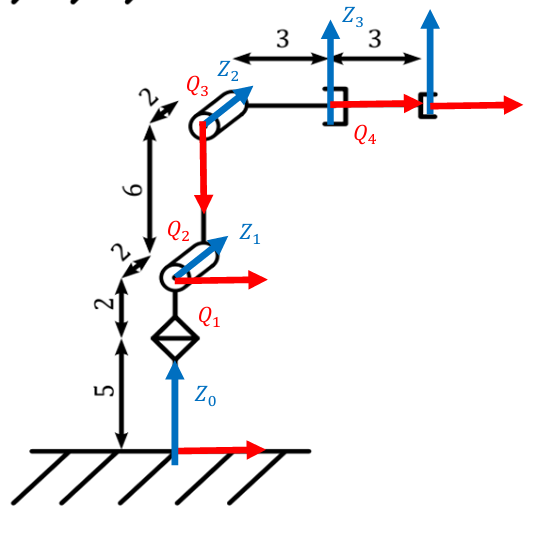
\includegraphics[width=0.4\textwidth]{Ej52.png}%
		\label{fig:ej52}
	}
	\caption{Ejercicio 5: Robot 9}
	\label{fig:Robot9}
\end{figure}
\begin{figure}[H]
	\centering
	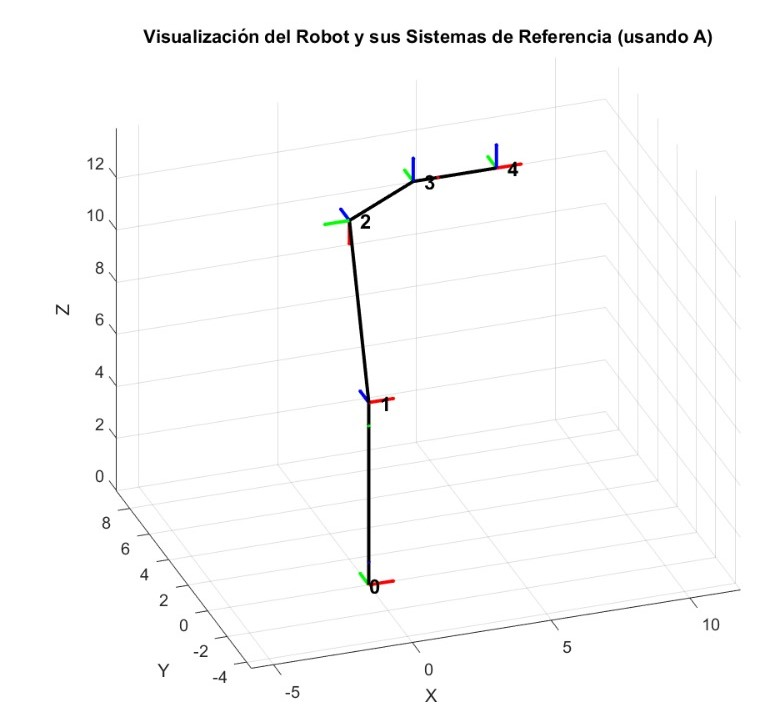
\includegraphics[width=0.6\textwidth]{img/Ej53.jpg}
	\caption{Robot 9 en MATLAB.}
	\label{fig:Robot9matlab}
\end{figure}

%-------------------------------------------
% Bibliografía
%-------------------------------------------
%\bibliographystyle{IEEEtran}  % Estilo de bibliografía IEEE
% La bibliografía se tomará del archivo "fuentes.bib"
%\bibliography{fuentes}
	
\end{document}
